\section{System Architecture}

The software is built on ROS2 and organized as an event-driven modular system. A central
\texttt{App} owns a typed \texttt{EventBus} for zero-coupling inter-component messaging
and a \texttt{ConfigManager} that hot-reloads TOML configuration files at runtime.

\section{Kinematics and Odometry}

A differential drive kinematic model converts encoder tick counts to linear wheel displacements
and integrates them into a 2D pose $(x, y, \theta)$. Velocity commands $(v, \omega)$ are
inverted to individual wheel setpoints regulated by PID controllers via PWM. An exponential
low-pass filter ($\tau{=}0.1\,\text{s}$) smooths the reported twist.

\section{SLAM and Localization}

\subsection{Occupancy Grid Mapping}

The environment is a $200{\times}200$ cell grid at 5\,cm resolution. Each LiDAR scan is
integrated via Bresenham ray-casting: traversed cells are marked \textit{free}, hit cells
\textit{occupied}, with probabilities clamped to prevent false certainty.

\subsection{Gauss-Newton Scan Matching}

Given pose $\mathbf{x}{=}(x,y,\theta)^\top$, each scan point is transformed to the world
frame and the occupancy value retrieved by bilinear interpolation. Gauss-Newton iterations
minimize $\sum_i(1{-}m(\mathbf{p}_i))^2$, accumulating the Hessian $\mathbf{H}{=}\mathbf{J}^\top\mathbf{J}$
and applying the correction $\Delta\mathbf{x}{=}\mathbf{H}^{-1}\mathbf{J}^\top\mathbf{r}$.
Match confidence is derived from the eigenvalue structure of $\mathbf{H}$.

\subsection{Monte Carlo Localization}

Symmetric corridors create pose ambiguity. MCL \cite{wiki_monte_carlo_localization} maintains
a pool of hypotheses, each refined by the scan matcher, governed by a four-state machine
(\textit{Initializing} $\to$ \textit{Stable} $\to$ \textit{Degraded} $\to$ \textit{Lost}).
On degradation, new hypotheses are spawned by perturbing the best pose within
${\pm}0.75\,\text{m}$ XY and ${\pm}\pi$ rotation; a 10\,s lost timeout triggers a full map
reset. Fig.~\ref{fig:mcl} shows the hypothesis cloud during an active localization event.

\begin{figure}[htbp]
    \centering
    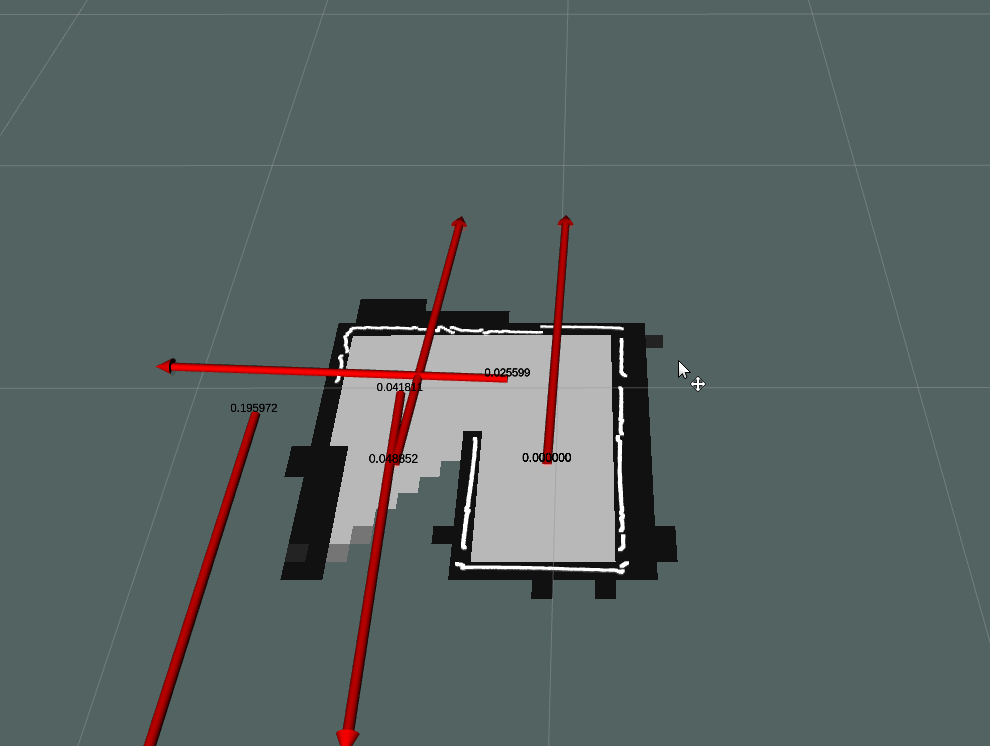
\includegraphics[width=0.85\columnwidth]{images/monte-carlo-localization.png}
    \caption{MCL visualization in RViz2. The displayed text is computed from the likelihood field and is shown in meters.}
    \label{fig:mcl}
\end{figure}

\subsection{Likelihood Field (Attempted)}

A likelihood field—an exponential distance transform of the occupied cells—was developed as an
alternative hypothesis scoring function. Fig.~\ref{fig:distance_field} illustrates the field
over a partially explored map.

\begin{figure}[htbp]
    \centering
    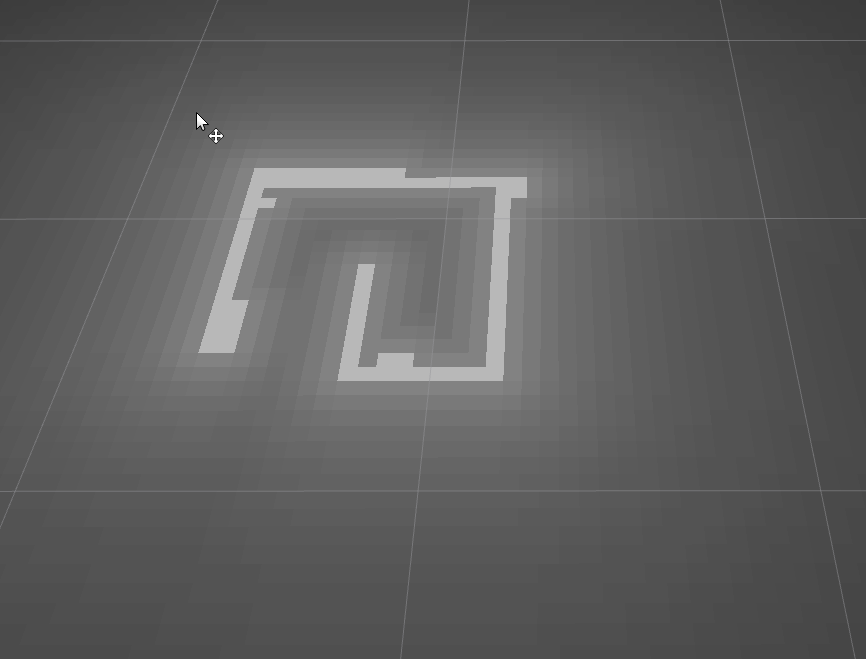
\includegraphics[width=\columnwidth]{images/distance-field-map.png}
    \caption{Likelihood field derived from the occupancy grid using exponential distance scaling.
        Bright regions correspond to locations close to occupied cells (high likelihood),
        while darker regions indicate increasing distance from obstacles (low likelihood).
        The field values are normalized to the range $[0,1]$.}
    \label{fig:distance_field}
\end{figure}

The method improved robustness in slow, controlled experiments but was sensitive to rapid rotations 
and the 5 Hz LiDAR update rate, occasionally producing misleading scores during fast maneuvers. It was 
excluded from the final real-world evaluation, as the Gauss-Newton matcher alone provided sufficient stability 
at operational speeds. In recovery cases, eigenvalue-based confidence degraded quickly and often led to 
loss of tracking and rescan triggers, whereas the likelihood-based score typically recovered after a brief 
loss and returned to a stable pose.

\section{Navigation}

\subsection{Corridor-Based Maze Navigation}

At each 10\,ms tick, \texttt{MazeEngine} casts 9 rays per side (${\pm}20°$). PCA fits wall
segments; two walls are accepted when their directions are similar.
A PD controller drives the heading error relative to the wall bisector; forward speed is
modulated by $v = v_{\max}\cdot\mathrm{clamp}(d_\text{front}/d_\text{corridor},0,1)^2$.
Junction detection triggers a \textit{Turning} state executing a 90°/180° PI-controlled rotation.
Fig.~\ref{fig:corridor} shows the debug view from the final evaluation run.

\begin{figure}[htbp]
    \centering
    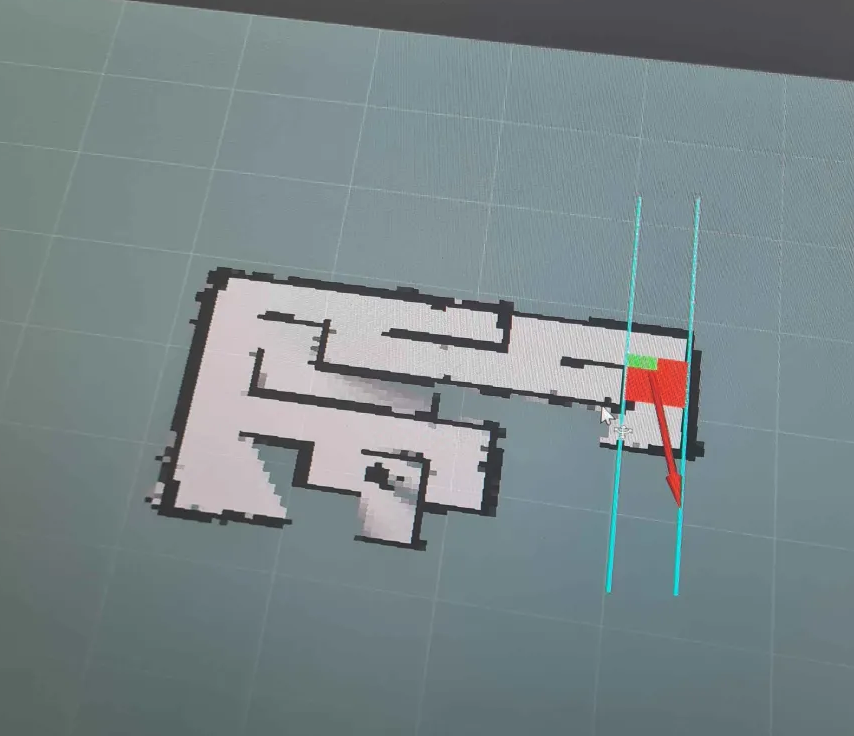
\includegraphics[width=0.85\columnwidth]{images/corridor-navigation.png}
    \caption{Corridor navigation debug view. Green lines: PCA-fitted walls.
             Yellow rays: junction detection casts.}
    \label{fig:corridor}
\end{figure}

\subsection{Dynamic Window Pure Pursuit (DWPP)}

A DWPP navigator \cite{arxiv2601_15006} samples $(v,\omega)$ candidates within the reachable dynamic window, 
forward-simulates each trajectory, and scores them by lookahead distance and heading alignment. Parameter 
tuning was still in progress and was abandoned before completion due to unfinished fine-tuning of variables. 
The approach was evaluated in a hybrid Unity+ROS2 simulation bridge designed for safe parameter exploration. 
Although not carried through to final evaluation, this method has a notable potential advantage: if fully realized, 
it could enable the robot to avoid costly 180-degree in-place rotations by allowing more natural reverse motion, 
improving efficiency in constrained corridor navigation.

\begin{figure}[htbp]
    \centering
    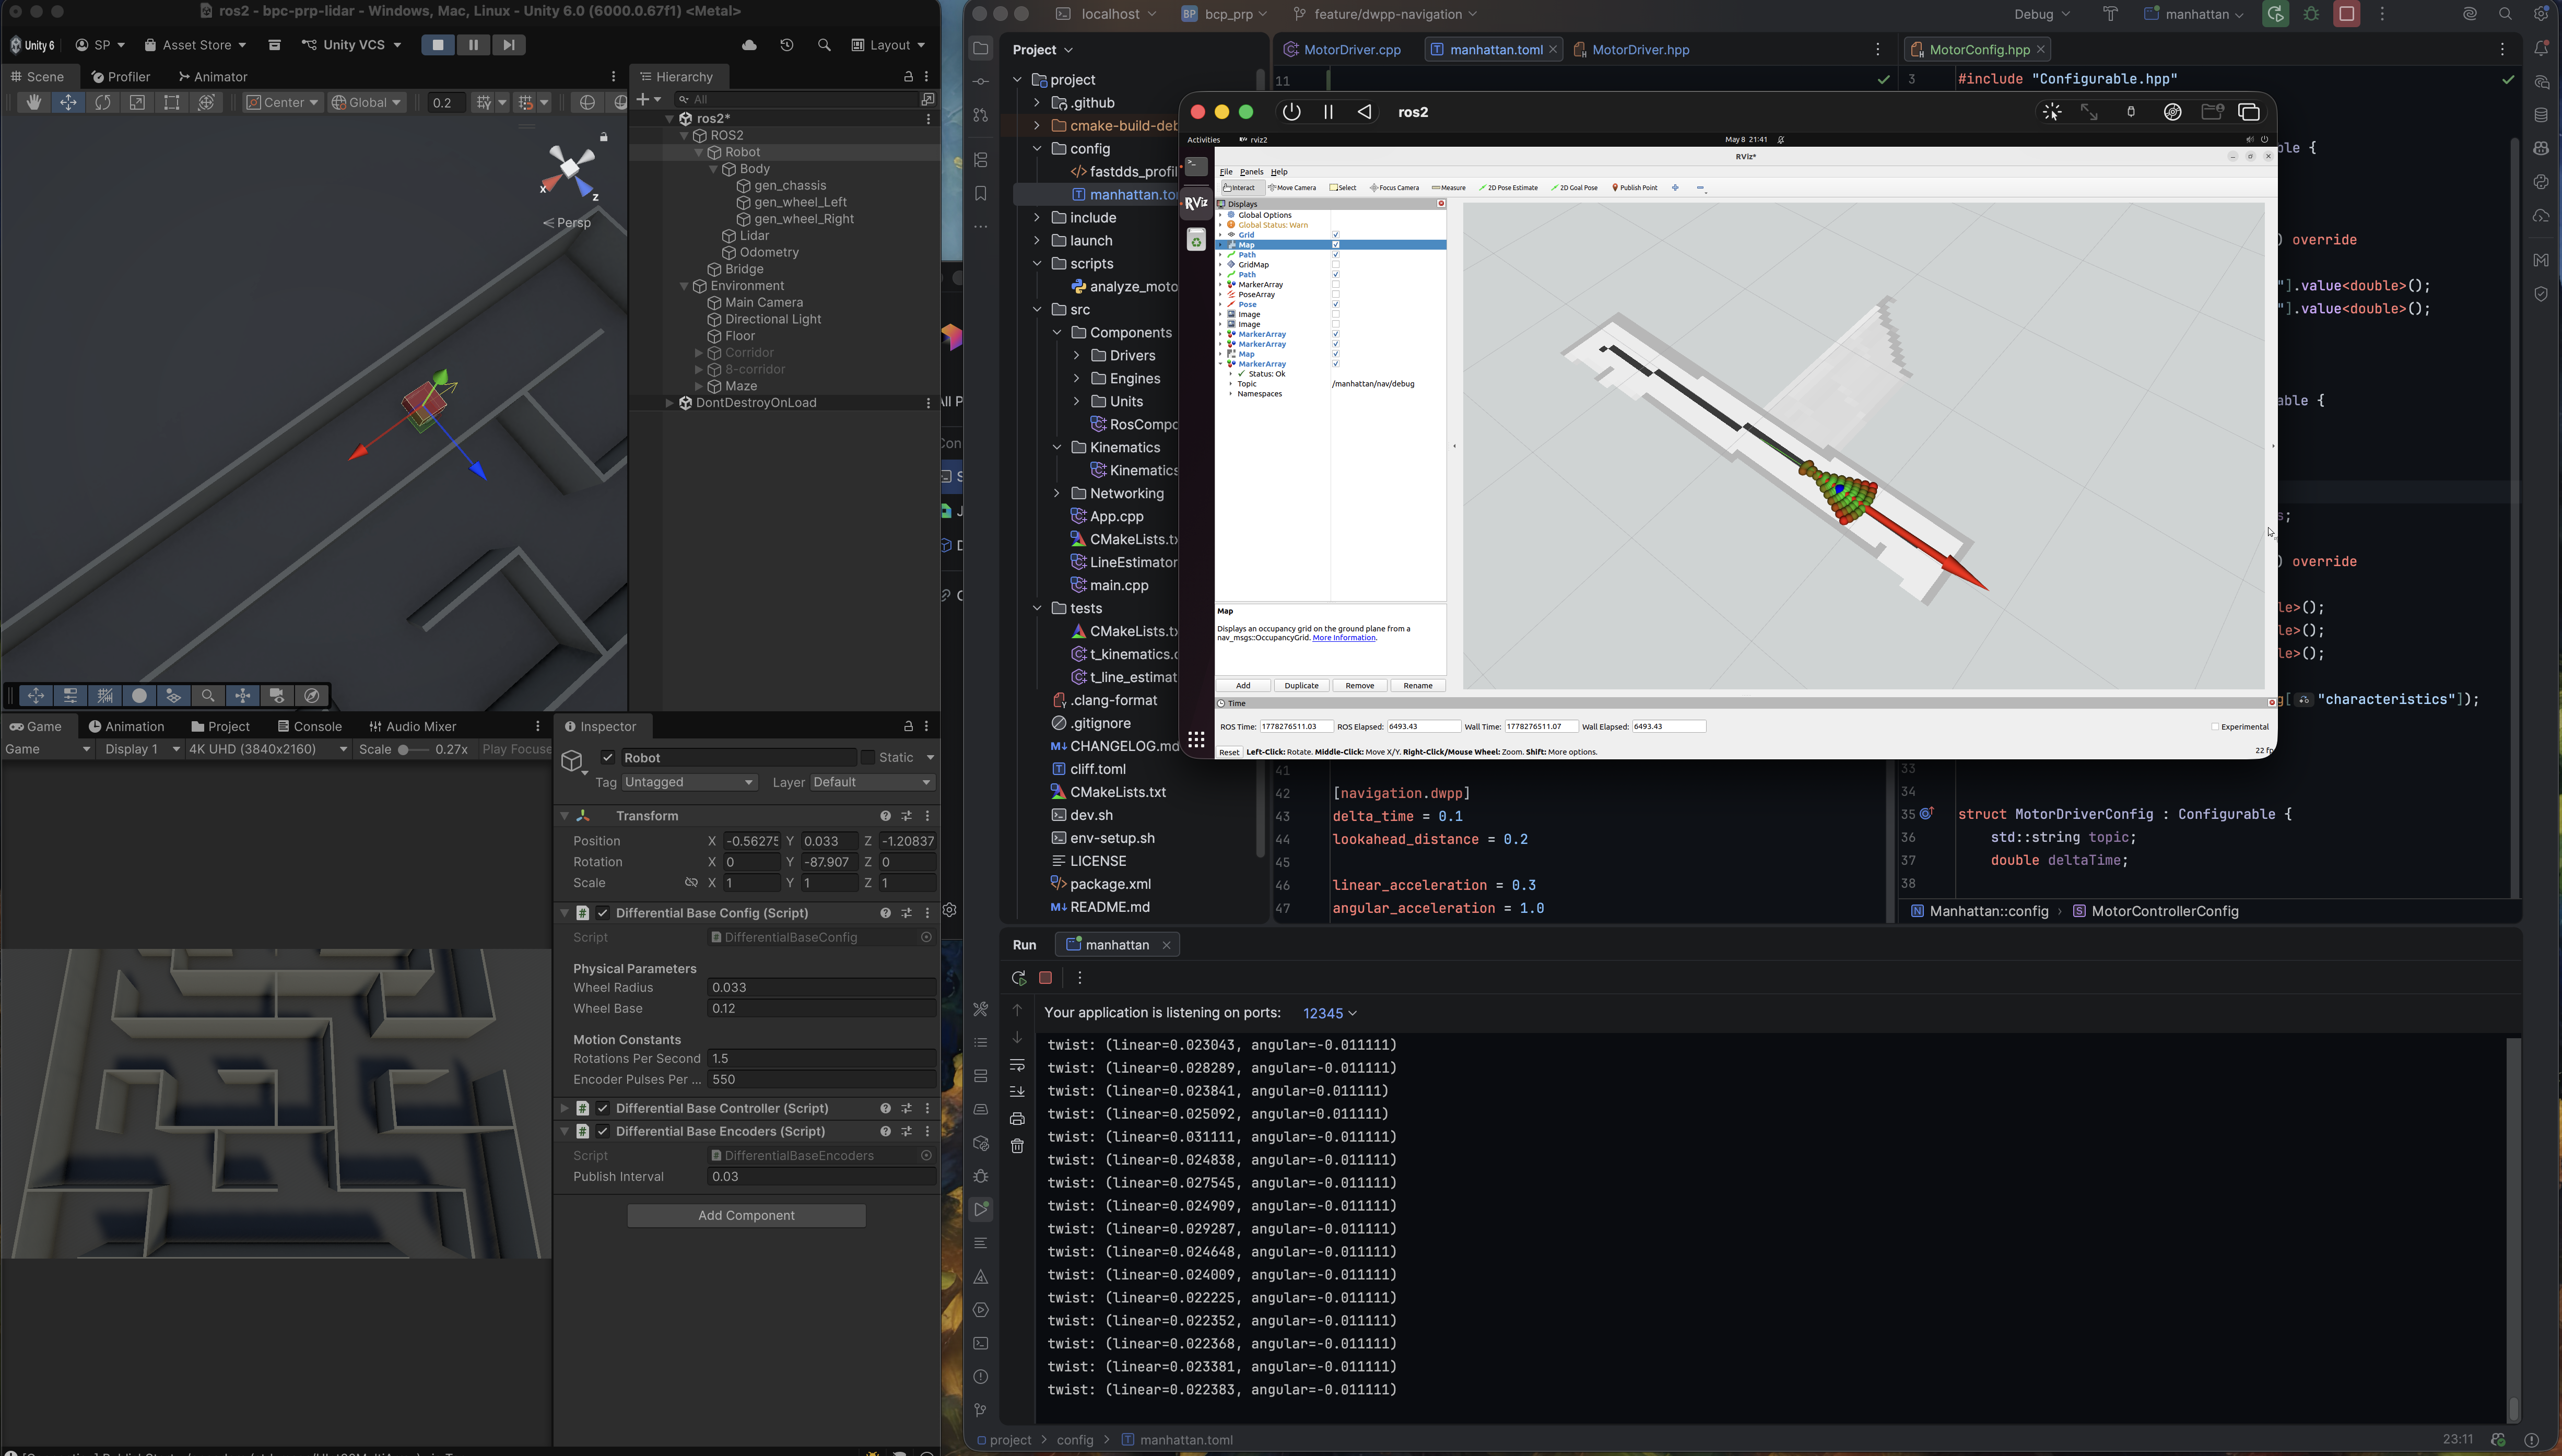
\includegraphics[width=\columnwidth]{images/unity-dwpp.png}
    \caption{DWPP tuning in the Unity simulation environment. The RViz2 overlay shows a
             $10{\times}10$ candidate velocity grid. Color (red$\to$green) encodes score;
             the virtual robot ran live ROS2 software against Unity physics.}
    \label{fig:dwpp}
\end{figure}

\subsection{Map Corruption}

Fast sudden changes of angular velocity caused little fizzyness and lost of robots orientation in environment.
The degenereted map structure caused Gauss-Newton confidence to decrese which led to map corruption as conflicting
scans were integrated at incorrect poses (Fig.~\ref{fig:broken}).

\begin{figure}[htbp]
    \centering
    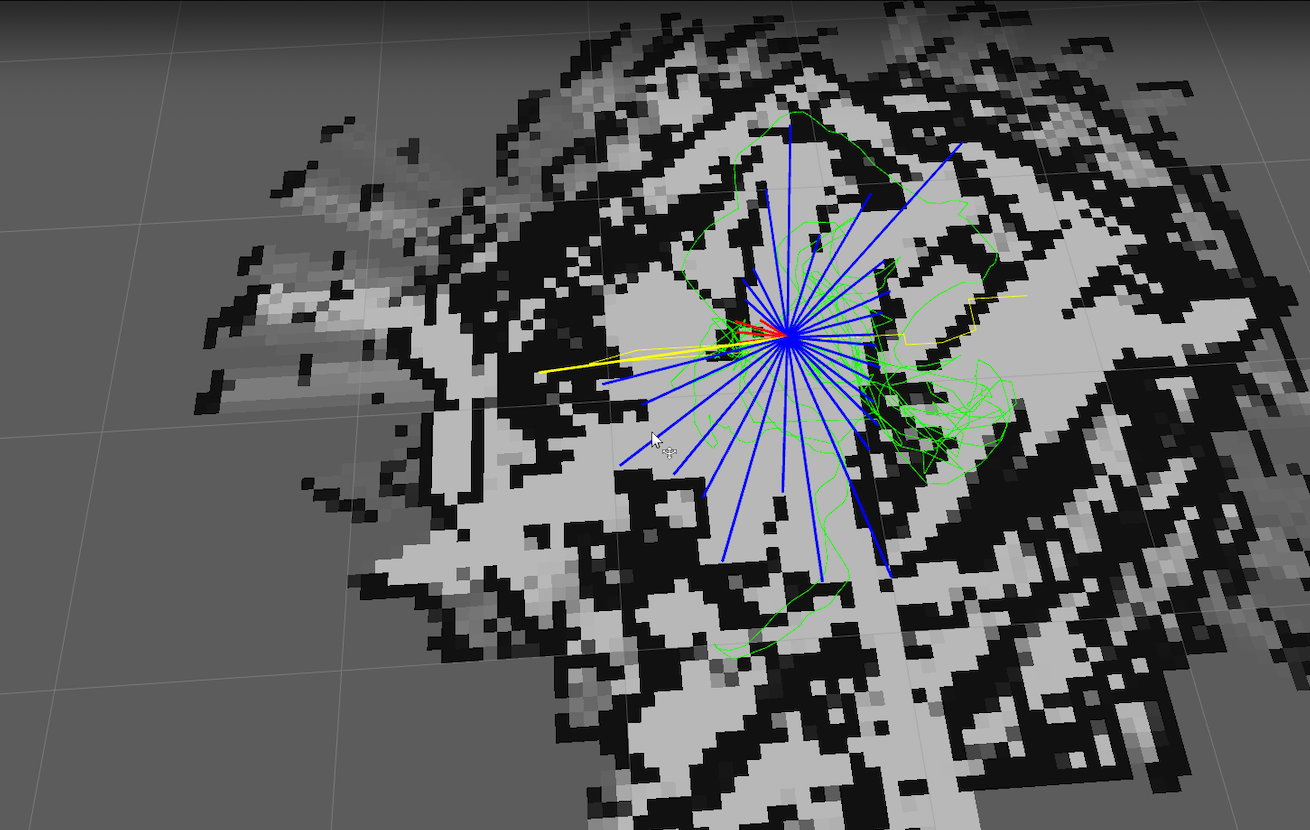
\includegraphics[width=\columnwidth]{images/broken-map.png}
    \caption{Corrupted occupancy grid resulting from localization failure in an open space.
             Multiple conflicting scan integrations create ghost obstacles and erase real walls,
             while the system attempts further recovery—making the map progressively worse.}
    \label{fig:broken}
\end{figure}

After refining the MCL confidence thresholds and hypothesis management, the open-space scenario
became paradoxically more stable than narrow corridors: the larger field of view provided more
LiDAR return points per scan, yielding a richer Hessian and higher scan-matcher confidence
(Fig.~\ref{fig:open}).

\begin{figure}[htbp]
    \centering
    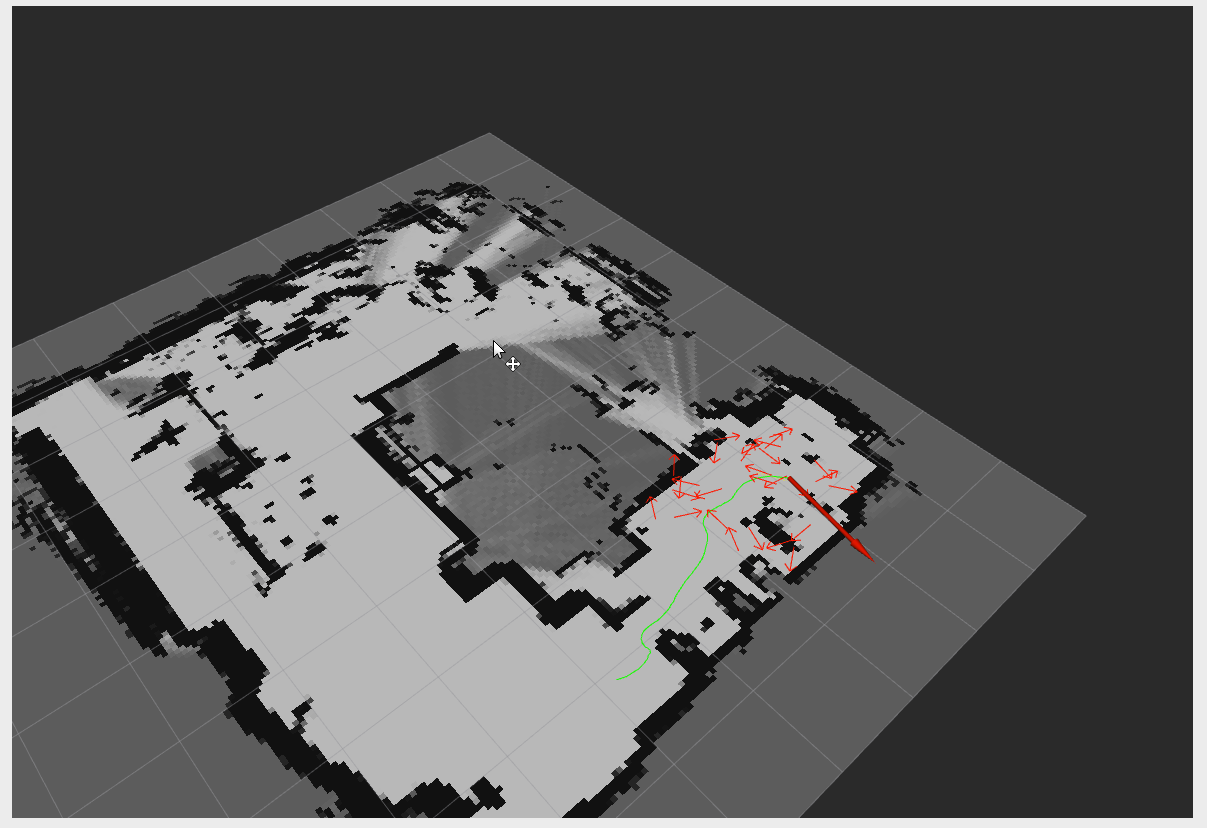
\includegraphics[width=\columnwidth]{images/open-space.png}
    \caption{Robot navigating an open space after MCL refinement. The occupancy grid remains
             consistent despite the initially problematic sparse, symmetric environment.}
    \label{fig:open}
\end{figure}
